% Created 2022-01-09 Sun 18:05
% Intended LaTeX compiler: pdflatex
\documentclass[a4paper,12pt]{article}
\usepackage[utf8]{inputenc}
\usepackage[T1]{fontenc}
\usepackage{graphicx}
\usepackage{grffile}
\usepackage{longtable}
\usepackage{wrapfig}
\usepackage{rotating}
\usepackage[normalem]{ulem}
\usepackage{amsmath}
\usepackage{textcomp}
\usepackage{amssymb}
\usepackage{capt-of}
\usepackage{hyperref}
\documentclass{article}
\usepackage{here}
\usepackage{xcolor}
\usepackage{amsmath}
\usepackage{parskip}
\renewcommand\arraystretch{1.4}
\usepackage[margin=1in]{geometry}
\usepackage{minted}
\usepackage{multicol}
\definecolor{bg}{rgb}{0.95,0.95,0.95}
\newminted{c}{fontsize=\footnotesize,frame=single,framesep=2mm}
\usepackage[demo]{graphicx}
\usepackage{subcaption}
\usepackage{caption}
\DeclareCaptionFormat{empty}{}
\captionsetup[subfigure]{labelformat=empty}
\newminted{text}{breaklines,fontsize=\footnotesize,frame=single,framesep=2mm}
\author{Fatih Kaan Salgır - 171044009}
\date{}
\title{CSE321 - Introduction to Algorithms - HW5}
\hypersetup{
 pdfauthor={Fatih Kaan Salgır - 171044009},
 pdftitle={CSE321 - Introduction to Algorithms - HW5},
 pdfkeywords={},
 pdfsubject={},
 pdfcreator={Emacs 27.2 (Org mode 9.5)}, 
 pdflang={English}}
\begin{document}

\maketitle

\section*{1}
\label{sec:org7ec7ef7}
\subsection*{a)}
\label{sec:org8e0d48c}
At any position, the maximum profit is either the element at the position or it is combined with previous cluster with maximum profit.
By applying this to the algorithm, iteratively, we can calculate the local maximum of the cluster, and then combine them to obtain maximum profit.
\begin{flalign*}
& C(n) = \sum_{i=0}^n 1 \in \Theta(n), \textrm{ where $n$ is the size of the array} &
\end{flalign*}
Application of the dynaminc programming doesn't affect the space complexity.


\subsection*{b)}
\label{sec:orge042520}
In brute-force approach the complexity is \(\Theta(n^2)\), in divide \& conquer approach the complexity is \(\Theta(n \log(n))\).
The dynamic programming approach can be considered as improved version of the brute-force version,
since it eliminates the checking of all possible sub-clusters but still using the previously calculated values.
And we have \(\Theta(n)\) complexity, which is the most efficient one among three algorithms.

\section*{2}
\label{sec:orgca08cc4}

The algorithm calculates the maximum profit for each length starting from 0.
For the subsequent values, the prior value is memoized.
This decreases the runtime of the inner loop drastically.
Since it is iterated over the first \(n\) element of the array, where \(n\) is the initial length,
the complexity algorithm doesn't depend on the size of the price array but only the length of the candy.
If we wouldn't implement dynamic programming;
\begin{flalign*}
& C(n) = \sum_{i=0}^n \sum_{j=0}^i 1 \in \Theta(n^2), \textrm{ where $n$ is the initial length of the candy} &
\end{flalign*}
With memoization the time complexity decreases to linear time (it is demonstrated in Figure 2).
Space complexity is also only dependant on given length which is \(\Theta(n)\), since it is memoized the maximum price corresponding to given length.


\begin{figure}[htbp]
\centering
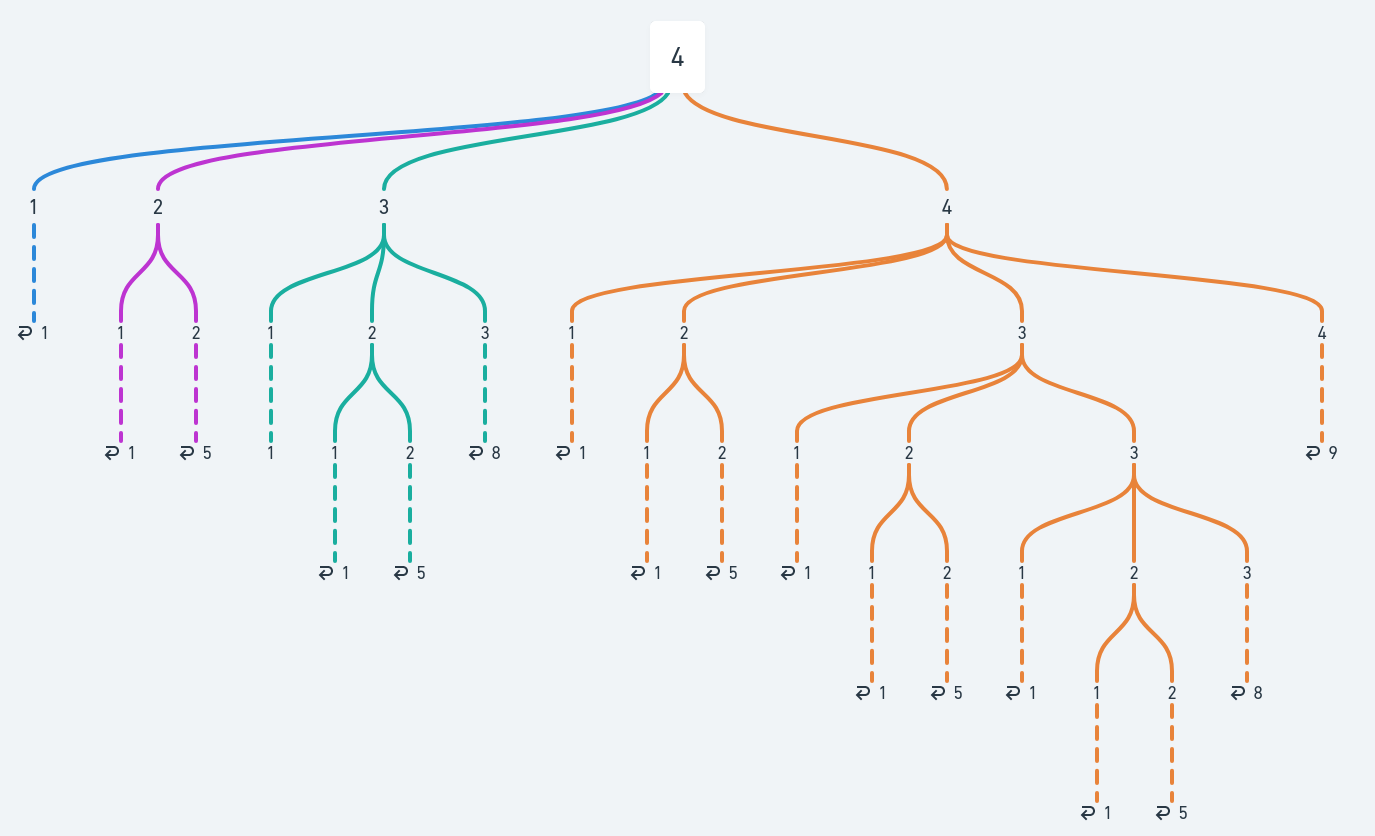
\includegraphics[width=400px]{org-img/2/2022-01-08_18-22-48_screenshot.png}
\caption{Example: length = 4, without using memoization}
\end{figure}


\begin{figure}[htbp]
\centering
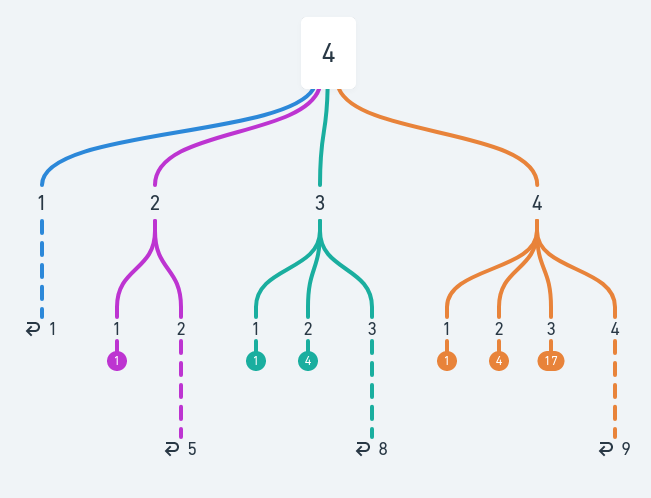
\includegraphics[width=200px]{org-img/2/2022-01-08_18-24-33_screenshot.png}
\caption{Example: length = 4, dynamic programming with memoization}
\end{figure}


\newpage

\section*{3}
\label{sec:orgefffd79}

First the cost of the cheese, ratio of price to weight, is calculated.
At each step of the algorithm, the cheese with maximum cost is chosen, which is locally optimal choice at each stage.
In order to choose the cheese with maximum cost, the array is sorted by cost.
Both calculating the costs, and choosing among them takes linear time.
Sorting ideally takes \(\Theta(n \log(n))\) time.
In total we have \(\Theta(n \log(n))\) time complexity.
\begin{flalign*}
& C(n) \in \Theta(n \log(n) + n + n) = \Theta(n \log(n)) &
\end{flalign*}
However, this sorting can lead unnecessary complexity if we have low capacity but higher number of cheese types.
Since, it sorts all array, but we need only first \(n\) number of maximum cost values.
So, one optimization might be getting the maximum value at each step.

\section*{4}
\label{sec:org76ef8cc}

The optimal choice of the greedy algorithm is finding the earliest finished course,
and removing the overlapped courses with the earliest finished course.
Finding the earliest is basically finding the minimum element in an array which takes linear time.
Removing the overlapped courses also takes linear time.
At worst case where we don't have overlapping course, the number of courses is getting decreased by 1 at each step.
That leads to \(\Theta(n^2)\) complexity.
However, in an average case, the removal of overlapping courses propagates the next step, which decreases the running time drastically.
\begin{flalign*}
& C_{worst}(n) = \sum_{i=0}^n \sum_{j=0}^i 1 \in \Theta(n^2), \textrm{ where $n$ number of courses} &
\end{flalign*}

\newpage
\end{document}
